\subsection{Link optimizations}
At first our link did not work. From simulations with equalization turned on and off and observing the eye diagram at the receiver input we could see that our equalization closed the eye instead of improving it. Debugging the schematics revealed that we implemented the tap with a positive sign instead of a negative sign and as result amplified the ISI of this cursor instead of canceling it. After changing the sign the equalization worked as expected.\\
After that we still got a lot of bit errors. As the input of the receiver was sufficient for the faulty bits we took a closer look at the intermediate signals in the receiver circuit. We figured out that the signal after our track-and-hold followed the input perfectly in the track phase. In the hold phase the differential signal was still maintained but the common mode of it made a significant step down towards the ground potential. Looking at the output of the following VOA in our design showed that this low common mode in the hold phase was to low for the amplifier to work and as consequence it only amplified the input signal in the track phase but not the hold phase, see figure \ref{fig:track_and_hold_problem} for the signals.

\begin{figure}[H]
  \centering
  {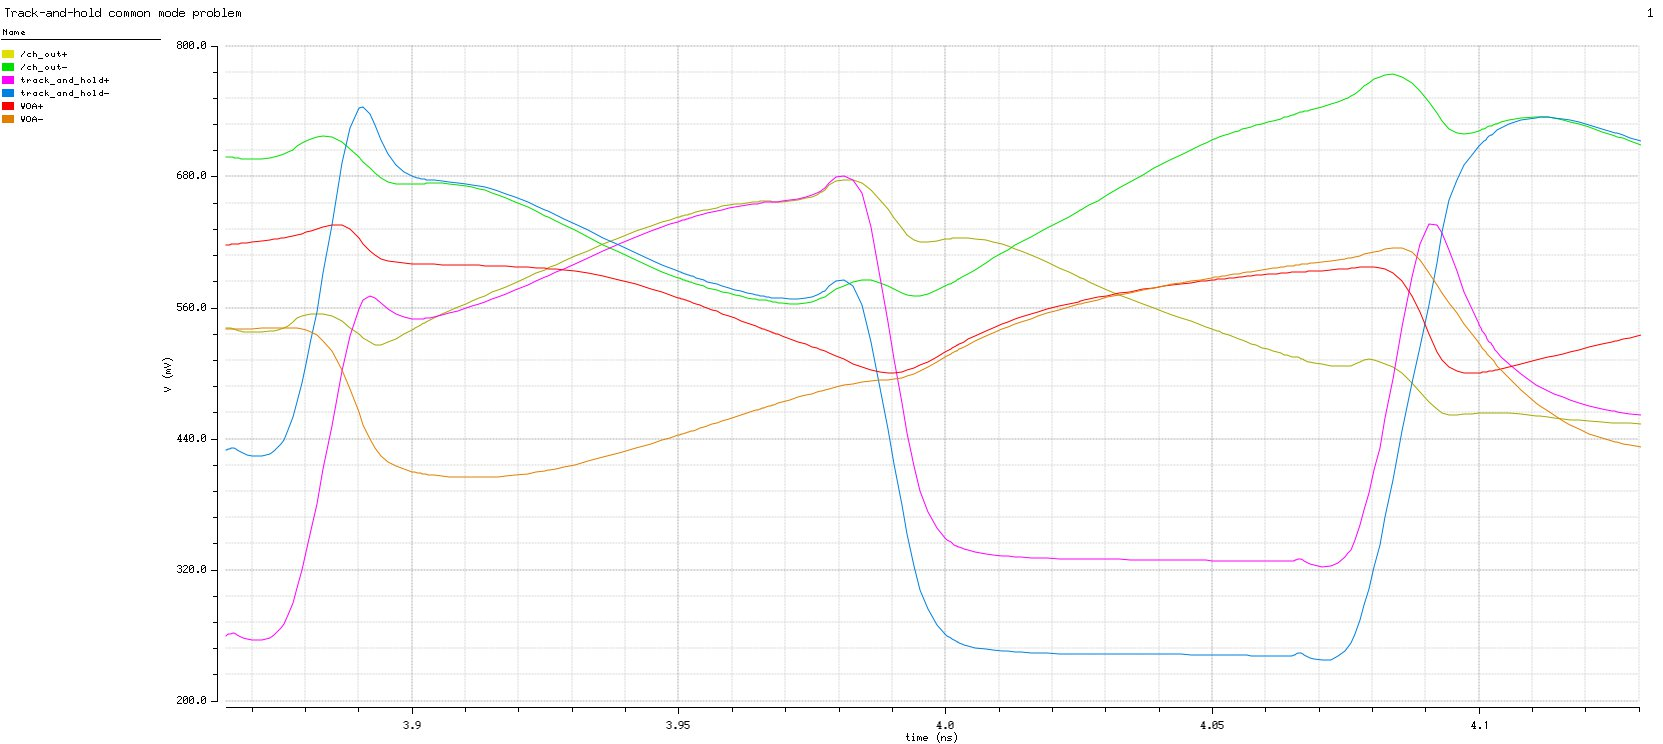
\includegraphics[scale=0.4]{img/track_and_hold_problem.png}}
  \caption{Track-and-hold common mode problem}
  \label{fig:track_and_hold_problem}
\end{figure}

This resulted in only half the time for the outputs to settle and would require double the bandwith for this amplifier than what we designed it for. This problem occured as we only used parasitic capacitances to implement the track-and-hold capacitance. The important capacitances here are the gate-source capacitance of the VOA input and the drain-bulk capacitance of the track-and-hold transistor. When the circuit now enters the hold phase the input is almost floating and only connected to these capacitances. As the source terminal of the VOA steers to ground now, the bulk is connected to $\overline{clk}$ and the voltage over the capacitors stays constant, the potential at the other terminal goes down. In other words, the reference potential changes.\\
To overcome this problem we added an extra capacitance of \unit[20]{fF} to the track-and-hold. This is approximatly five times larger than the parasitic capacitances and always connected to the same reference potential (GND), therefore the output stays almost constant between track and the hold phase.
